{\color{red} Realizar un procedimiento con \textbf{wildcard} que me permita seleccionar los primeros \texttt{40} ips impares a partir de la ip \texttt{48}. Red Base: \texttt{10.10.0.0}} \\

\noindent
\begin{minipage}[t]{.5\textwidth}
\textbf{Wildcard \#1}: \fbox{\texttt{0.0.0.14} }
	
	\begin{center}
	
	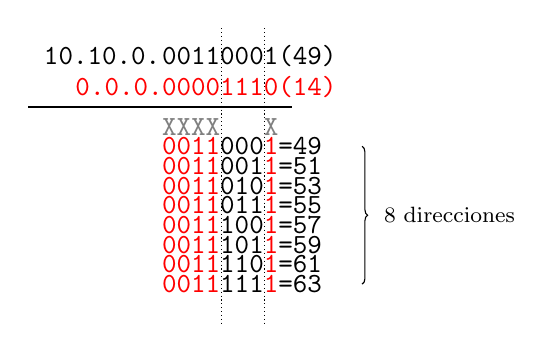
\begin{tikzpicture}

\draw(-0.1,-0.25) -- (3.25,-0.25);


%LINEA PUNTEADA
\draw[densely dotted] (2.35,0.75) -- (2.35,-3);
\draw[densely dotted] (2.9,0.75) -- (2.9,-3);


\node[text width=3cm] at (1.6,0.4) 
    {\texttt{10.10.0.}};
\node[text width=3cm] at (3.1,0.4) 
    {\texttt{00110001(49)}};
%WILDCARD
\node[text width=3cm] at (2,0) 
    {{\color{red}\texttt{0.0.0.}}};
\node[text width=3cm] at (3.1,0) 
    {{\color{red}\texttt{00001110(14)}}};


\node[text width=3cm] at (3.1,-0.5) 
    { {\color{gray}\texttt{XXXX\phantom{XXX}X}}};

\node[text width=3cm] at (3.1,-0.75) 
    {\texttt{{\color{red}0011}000{\color{red}1}=49}};

\node[text width=3cm] at (3.1,-1) 
    {\texttt{{\color{red}0011}001{\color{red}1}=51}};

\node[text width=3cm] at (3.1,-1.25) 
    {\texttt{{\color{red}0011}010{\color{red}1}=53}};    

\node[text width=3cm] at (3.1,-1.5) 
    {\texttt{{\color{red}0011}011{\color{red}1}=55}};

\node[text width=3cm] at (3.1,-1.75) 
    {\texttt{{\color{red}0011}100{\color{red}1}=57}};

\node[text width=3cm] at (3.1,-2) 
    {\texttt{{\color{red}0011}101{\color{red}1}=59}};

\node[text width=3cm] at (3.1,-2.25) 
    {\texttt{{\color{red}0011}110{\color{red}1}=61}};

\node[text width=3cm] at (3.1,-2.5) 
    {\texttt{{\color{red}0011}111{\color{red}1}=63}};

\draw [decorate,decoration={brace,amplitude=2pt,mirror,raise=4pt},yshift=0pt]
(4,-2.5) -- (4,-0.75)  node [black,midway,xshift=1.25cm] {\footnotesize 8 direcciones};



\end{tikzpicture}
\end{center}
	
\end{minipage}% <---------------- Note the use of "%"
\begin{minipage}[t]{.5\textwidth}
	
	\textbf{Wildcard \#2}:  \fbox{\texttt{0.0.0.62} }
	
	\begin{center}
	
	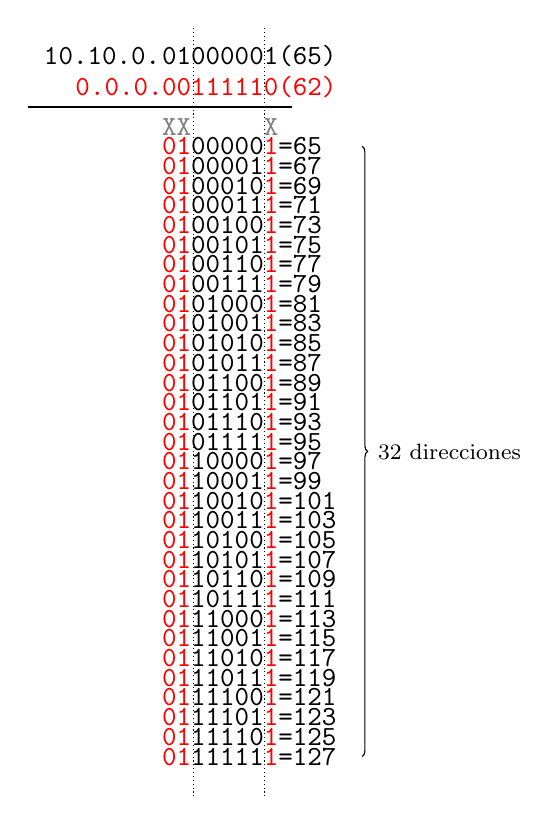
\begin{tikzpicture}

\draw(-0.1,-0.25) -- (3.25,-0.25);


%LINEA PUNTEADA
\draw[densely dotted] (2,0.75) -- (2,-9);
\draw[densely dotted] (2.9,0.75) -- (2.9,-9);


\node[text width=3cm] at (1.6,0.4) 
    {\texttt{10.10.0.}};
\node[text width=3cm] at (3.1,0.4) 
    {\texttt{01000001(65)}};
%WILDCARD
\node[text width=3cm] at (2,0) 
    {{\color{red}\texttt{0.0.0.}}};
\node[text width=3cm] at (3.1,0) 
    {{\color{red}\texttt{00111110(62)}}};


\node[text width=3cm] at (3.1,-0.5) 
    { {\color{gray}\texttt{XX\phantom{XXXXX}X}}};

\node[text width=3cm] at (3.1,-0.75) 
    {\texttt{{\color{red}01}00000{\color{red}1}=65}};

\node[text width=3cm] at (3.1,-1) 
    {\texttt{{\color{red}01}00001{\color{red}1}=67}};

\node[text width=3cm] at (3.1,-1.25) 
    {\texttt{{\color{red}01}00010{\color{red}1}=69}};    

\node[text width=3cm] at (3.1,-1.5) 
    {\texttt{{\color{red}01}00011{\color{red}1}=71}};

\node[text width=3cm] at (3.1,-1.75) 
    {\texttt{{\color{red}01}00100{\color{red}1}=73}};

\node[text width=3cm] at (3.1,-2) 
    {\texttt{{\color{red}01}00101{\color{red}1}=75}};

\node[text width=3cm] at (3.1,-2.25) 
    {\texttt{{\color{red}01}00110{\color{red}1}=77}};

\node[text width=3cm] at (3.1,-2.5) 
    {\texttt{{\color{red}01}00111{\color{red}1}=79}};

\node[text width=3cm] at (3.1,-2.75) 
    {\texttt{{\color{red}01}01000{\color{red}1}=81}};    

\node[text width=3cm] at (3.1,-3) 
    {\texttt{{\color{red}01}01001{\color{red}1}=83}};  

\node[text width=3cm] at (3.1,-3.25) 
    {\texttt{{\color{red}01}01010{\color{red}1}=85}};  
    
\node[text width=3cm] at (3.1,-3.5) 
    {\texttt{{\color{red}01}01011{\color{red}1}=87}};  

\node[text width=3cm] at (3.1,-3.75) 
    {\texttt{{\color{red}01}01100{\color{red}1}=89}};  

\node[text width=3cm] at (3.1,-4) 
    {\texttt{{\color{red}01}01101{\color{red}1}=91}};  

\node[text width=3cm] at (3.1,-4.25) 
    {\texttt{{\color{red}01}01110{\color{red}1}=93}};  

\node[text width=3cm] at (3.1,-4.5) 
    {\texttt{{\color{red}01}01111{\color{red}1}=95}};  

\node[text width=3cm] at (3.1,-4.75) 
    {\texttt{{\color{red}01}10000{\color{red}1}=97}};  

\node[text width=3cm] at (3.1,-5) 
    {\texttt{{\color{red}01}10001{\color{red}1}=99}};  

\node[text width=3cm] at (3.1,-5.25) 
    {\texttt{{\color{red}01}10010{\color{red}1}=101}};  

\node[text width=3cm] at (3.1,-5.5) 
    {\texttt{{\color{red}01}10011{\color{red}1}=103}};  

\node[text width=3cm] at (3.1,-5.75) 
    {\texttt{{\color{red}01}10100{\color{red}1}=105}};  

\node[text width=3cm] at (3.1,-6) 
    {\texttt{{\color{red}01}10101{\color{red}1}=107}};  

\node[text width=3cm] at (3.1,-6.25) 
    {\texttt{{\color{red}01}10110{\color{red}1}=109}};  
    
\node[text width=3cm] at (3.1,-6.5) 
    {\texttt{{\color{red}01}10111{\color{red}1}=111}};  

\node[text width=3cm] at (3.1,-6.75) 
    {\texttt{{\color{red}01}11000{\color{red}1}=113}};  

\node[text width=3cm] at (3.1,-7) 
    {\texttt{{\color{red}01}11001{\color{red}1}=115}};  
    
\node[text width=3cm] at (3.1,-7.25) 
    {\texttt{{\color{red}01}11010{\color{red}1}=117}};   
    
\node[text width=3cm] at (3.1,-7.5) 
    {\texttt{{\color{red}01}11011{\color{red}1}=119}};      

\node[text width=3cm] at (3.1,-7.75) 
    {\texttt{{\color{red}01}11100{\color{red}1}=121}};   

\node[text width=3cm] at (3.1,-8) 
    {\texttt{{\color{red}01}11101{\color{red}1}=123}};   

\node[text width=3cm] at (3.1,-8.25) 
    {\texttt{{\color{red}01}11110{\color{red}1}=125}};
    
\node[text width=3cm] at (3.1,-8.5) 
    {\texttt{{\color{red}01}11111{\color{red}1}=127}};      

\draw [decorate,decoration={brace,amplitude=2pt,mirror,raise=4pt},yshift=0pt]
(4,-8.5) -- (4,-0.75)  node [black,midway,xshift=1.25cm] {\footnotesize 32 direcciones};


\end{tikzpicture}
\end{center}
\end{minipage}
\\{ }\\
En ambos casos el \textit{LSB} se marcó como cero debido a la condición de que tienen que ser impares. Se puede ver ademas que la cantidad de direcciones que admite son las 40 que plantea el problema.